\chapter{Determining Structural Correspondences}\label{background2}
In order to construct a structural generalization describing the commonalities and differences between ASTs of two given logged methods (LMs), I first needed to find structural correspondences between their nodes. The approach to determining correspondences proceeds in three steps: first, computing similarities between AST nodes (Section~\ref{jigsaw-similarity}); second, determining potential structural correspondences between nodes (Section~\ref{jigsaw-corr}); third, creating an extended form of AST to allow the insertion of variables in place of any nodes in the tree structure(Section~\ref{auast}).

%To construct an anti-unified structure, I first need to create an extended form of the CAST structure, called \emph{anti-unifier ASTs} (AUASTs), to allow the insertion of variables in place of any nodes in the tree structure (Section~\ref{auast})

To implement the approach, I needed a concrete framework for constructing and manipulating ASTs. The \name{Eclipse} integrated development environment provides such a framework in its \name{Java Development Tools} (JDT) component (as explained in Section~\ref{JDT}). I also utilized \name{Jigsaw} \cite{2008:fse:cottrell}, which is an existing framework for constructing an extended form of the AST structure, called CAST, where each node holds a list of candidate correspondence connections (as described in Section~\ref{Jigsaw}). Then, I extended the CAST structure to \emph{anti-unifier ASTs} (AUASTs) structure that would allow the creation of anti-unifier in a later step. To evaluate the effectiveness of Jigsaw to determining correspondences, I applied it on the ASTs of a sample set of logged Java methods and compared them in a pairwise manner. Section~\ref{jigsaw-assessment} describes my experimental setup, present my study, and discuss the results. I built atop this work in order to create anti-unifiers in a later phase.

%\RW{This goes later.} I built atop this work in order to create anti-unifiers.
%we or I???
% and a comparison of our tool with Jigsaw (Section~\ref{comparison-Jigsaw}).
%jEdit v4.2 pre 15 (2004)


%\subsection{Extracting the ASTs of LMs}\label{Jigsaw_usage}
%In order to describe the structure of \name{Java} methods that make use of logging calls in a program, we need to extract their ASTs (as described in Section~\ref{AST}).


\section{Computing similarity between nodes}  \label{jigsaw-similarity}
To compute similarity between AST nodes, I re-used a function developed by \citet{2008:fse:cottrell}, which first computes the number of common elements between the two nodes and then divides it by the size of the largest node, as described by the Equation~\ref{eq-jigsaw-sim}. \RW{I changed the formula because it made no sense before.}


\begin{equation}\label{eq-jigsaw-sim}
\id{similarity} = \frac{\id{matches}}{\max\{|\id{a}|, |\id{b}|\}}
\end{equation}


They compute the number of matched elements between the two AST nodes $\id{a}$ and $\id{b}$ via the \func{Determine-Matches} algorithm. As mentioned in Section~\ref{Jigsaw}, their approach only compares the nodes of identical or semantically equivalent types, thus the both input nodes are either leaf nodes or non-leaf nodes (Line~2). If they are of leaf nodes, the number of matches will be computed using the heuristics described in Section~\ref{Jigsaw} (Lines~3--4). If they are of non-leaf nodes, the children of the two subtrees $\id{a}$ and $\id{b}$ are compared exhaustively in a pairwise manner (Lines~5--16). For each child node of the subtree $\id{a}$, the highest similarity with any child node of the subtree $\id{b}$ is determined (Lines~6--14). All these maximum matches are summed up and returned as the number of common elements, which can be used to determine a potential structural correspondence between the two nodes (Line~15--19) as will be described in the following section.
%with a comparable type

\begin{algorithm}
 \caption{\func{Determine-Matches}($\id{a}$,$\id{b}$) computes the common elements ($\id{matches}$) between the two ASTs.}
  \label{simi}
  \begin{algorithmic}[1]
  \ComputeMatches
  \State $\id{matches} \gets 0$
  \If{$\func{Lookup-Comparator}(\id{type}[\id{a}],\id{type}[\id{b}]) $}
\If {$\id{a} \Instanceof \cons{Leaf-Node}$ }	
  \State $\id{matches} \gets  \func{matches}(\id{a},\id{b})$
  \ElsIf {$\id{a} \Instanceof \cons{Non-Leaf-Node}$ }	
 \For {$\id{childA} \in \id{children}[\id{a}]$}
		\State $\id{max} \gets 0$
		\For {$\id{childB} \in \id{children}[\id{b}]$}	
			\State $\id{matches} \gets  \func{Determine-Matches}(childA,childB)$
 		\If {$\id{matches} > \id{max}$ }	
 		\State $\id{max} \gets \id{matches}$	
		\EndIf
 \EndFor 	
	  \EndFor 	
	    \State $\id{matches} \gets  \id{matches} +  \id{max}$
 \EndIf
 \State \func{Create-Correspondence-Connection}($\id{a}$,$\id{b}$,$\id{matches}$)
 		\EndIf 		


 \Return $matches$
\end{algorithmic}
\end{algorithm}



\section{Determining potential correspondences}  \label{jigsaw-corr}

As discussed in Section~\ref{Jigsaw}, the proposed approach by \citet{2008:fse:cottrell} generates an augmented form of AST, called \emph{correspondence AST} (CAST), where each node holds a list of candidate correspondence connections. The \func{Create-Correspondence-Connection}($\id{a}$,$\id{b}$,$\id{matches}$) algorithm is used to create the CAST structure, which computes similarity between the two AST nodes using the Equation~\ref{eq-jigsaw-sim} (Line~1). If the similarity value is above a pre-determined threshold, a correspondence connection will be created and added to the list of correspondence connections of the corresponding nodes (Lines~2--6). As an example, Figure~\ref{fig:meth-ast-1} shows potential structural correspondence connections created via the application of \func{Determine-Matches} algorithm on the ASTs of Examples 1 and 2.


\begin{algorithm}
  \caption{\func{Create-Correspondence-Connection}($\id{a}$,$\id{b}$,$\id{matches}$) creates a candidate correspondence connection between the two AST nodes.}
  \label{computeMatches}
  \begin{algorithmic}[1]
  \DeterminePotentialCorrespondences
      %\For {$\id{nodeA} \in \id{a}$}
 	%	\For {$\id{nodeB} \in \id{b}$}
%\If{$\func{Lookup-Comparator}(\id{type}[\id{a}],\id{type}[\id{b}]) $}		
\State $\id{sim} \gets \id{matches} /\max\{{|\id{a}|, |\id{b}|}\}$	
 			\If {$sim > \cons{Threshold}$}	
 		\State $\id{corr} \gets \func{New-Correspondence-Connection}(\id{nodeA},\id{nodeB},\id{sim})$	
 \State $\func{Append}(\id{corrs}[\id{nodeA}],corr)$	
 \State $\func{Append}(\id{corrs}[\id{nodeB}],corr)$
 		\EndIf 		

 %		\EndIf 		

% \EndFor 	
%	  \EndFor 	
	
  \end{algorithmic}
\end{algorithm}



\begin{figure} [H]  \centering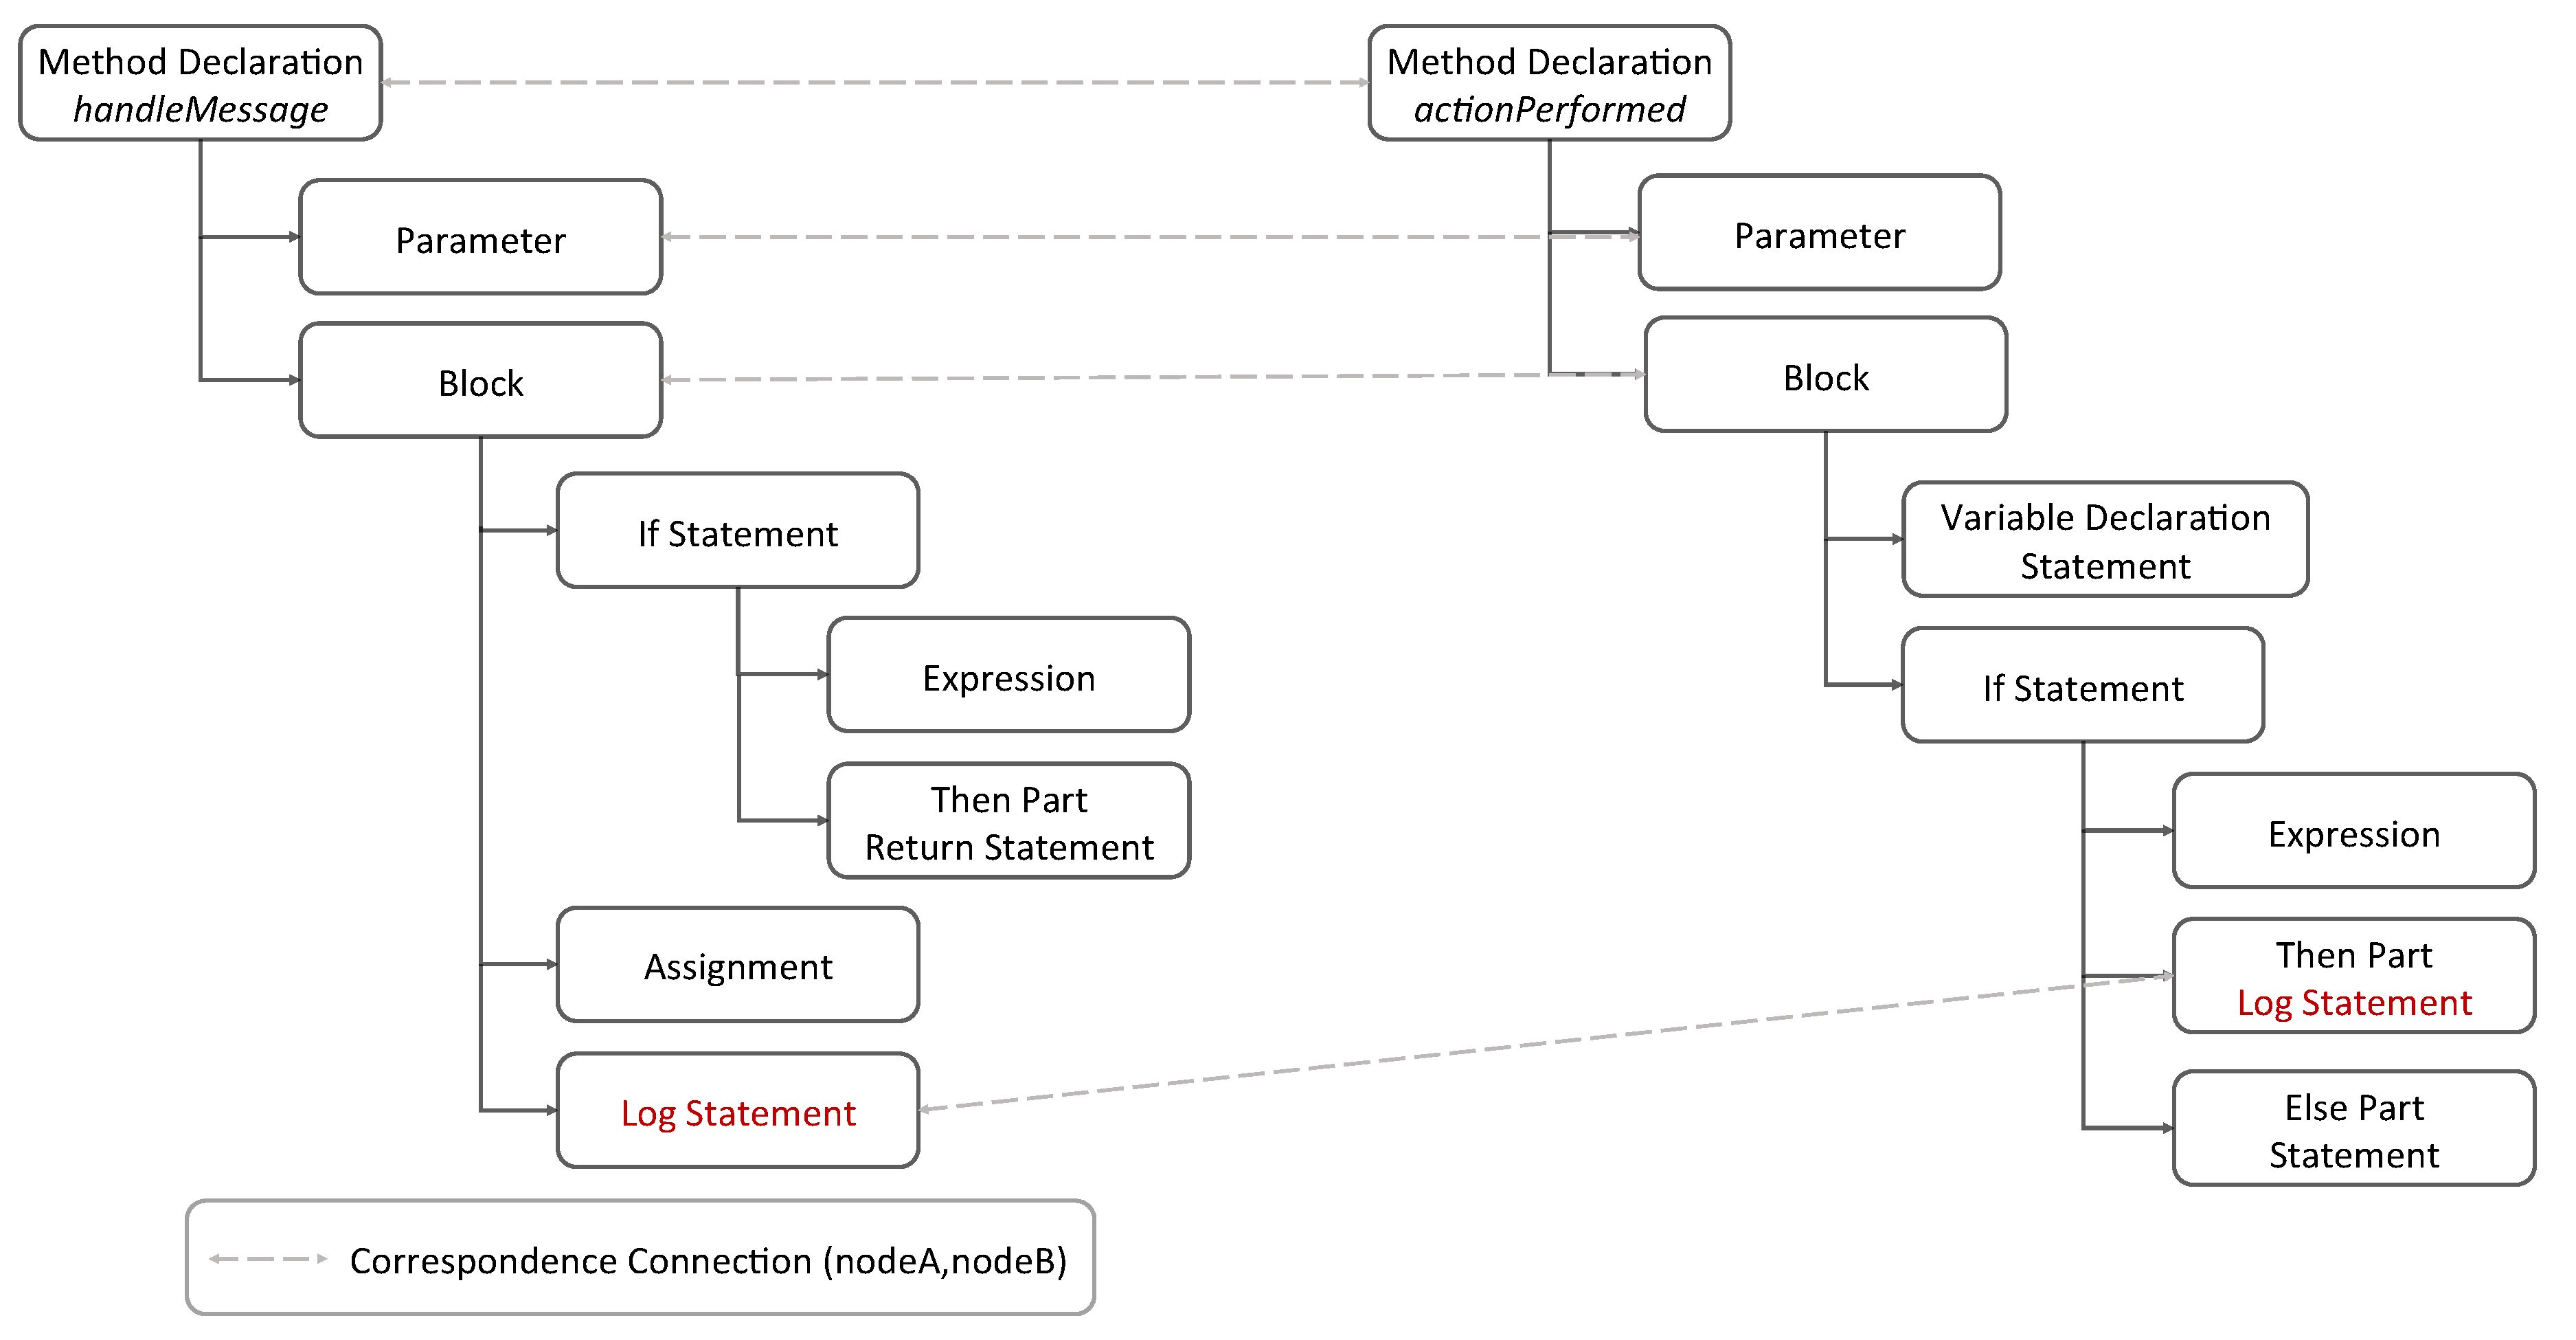
\includegraphics [width = \textwidth]{Drawing4/FirstCorr.pdf}
  \caption[Simple CAST structure of the examples in Figures~\ref{ch3-ex1} and~\ref{ch3-ex2}.]{Simple CAST structure of the examples in Figures~\ref{ch3-ex1} and~\ref{ch3-ex2}. The links between the CAST nodes indicate the structural correspondence connections.}
  \label{fig:meth-ast-1}
\end{figure}


%\begin{align}
%\Theta_1 = (W &\rightarrow \text{ \textsf{\small WARNING}},\nonumber\\
%X &\rightarrow \text{ \textit{methodCall}(\textit{simpleName}(\textsf{\small getClassName}), \textit{arguments}())},\nonumber\\
%Y &\rightarrow \text{ \textsf{\small "should extend EditPlugin not EBPlugin since it has an empty "}},\nonumber\\
%Z &\rightarrow \text{ \textit{methodCall}(\textit{simpleName}(\textsf{\small handleMessage}), \textit{arguments}())})\label{eq:theta1}\\
%\Theta_2 = (W &\rightarrow \text{ \textsf{\small ERROR}},\nonumber\\
%X &\rightarrow \text{ \NIL{}},\nonumber\\
%Y &\rightarrow \text{ \textsf{\small "Unknown action: "}},\nonumber\\
%Z &\rightarrow \text{ \textit{simpleName}(\textsf{\small actionName})})\label{eq:theta2}
%\end{align}
%
%%\item it can be mapped to our recursive definition of a term, where AST nodes and simple values may be viewed as function-symbols and constants, respectively
%
%\begin{figure}[p]
%\begin{small}
%\begin{tikzpicture}
%\node(a) at (4.25,10) {%
%\fbox{\parbox[b][][b]{3in}{%
%\text{\textit{methodCall}(}\\
%\text{\hspace*{1em}\textit{qualifiedName}(\textsf{\footnotesize Log}, \textit{simpleName}(\textsf{\footnotesize log})),}\\
%\text{\hspace*{1em}\textit{arguments}(}\\
%\text{\hspace*{2em}\textit{qualifiedName}(\textsf{\footnotesize Log}, \textit{simpleName}(\textit{W})),}\\
%\text{\hspace*{2em}\textit{thisExpression}(),}\\
%\text{\hspace*{2em}\textit{additionExpression}(\textit{X}, \textit{stringLiteral}(\textit{Y}), \textit{Z})))}}}%
%};
%\node(b) at (0,0) {%
%\fbox{\parbox[t][][b]{3.1in}{%
%\text{\textit{methodCall}(}\\
%\text{\hspace*{1em}\textit{qualifiedName}(\textsf{\footnotesize Log}, \textit{simpleName}(\textsf{\footnotesize log})),}\\
%\text{\hspace*{1em}\textit{arguments}(}\\
%\text{\hspace*{2em}\textit{qualifiedName}(\textsf{\footnotesize Log},}\\ \text{\hspace*{3em}\mbox{\textit{simpleName}(\textsf{\footnotesize WARNING})}),}\\
%\text{\hspace*{2em}\textit{thisExpression}(),}\\
%\text{\hspace*{2em}\textit{additionExpression}(}\\
%\text{\hspace*{3em}\textit{methodCall}(\textit{simpleName}(\textsf{\footnotesize getClassName}),}\\ \text{\hspace*{4em}\textit{arguments}()),}\\
%\text{\hspace*{3em}\textit{stringLiteral}(\textsf{\footnotesize " should extend ... "}),}\\
%\text{\hspace*{3em}\textit{methodCall}(\textit{simpleName}(\textsf{\footnotesize handleMessage}),}\\ \text{\hspace*{4em}\textit{arguments}()))))}}}%
%};
%\node(c) at (8.5,0.7) {%
%\fbox{\parbox[t][][b]{2.55in}{%
%\text{\textit{methodCall}(}\\
%\text{\hspace*{1em}\textit{qualifiedName}(\textsf{\footnotesize Log}, \textit{simpleName}(\textsf{\footnotesize log})),}\\
%\text{\hspace*{1em}\textit{arguments}(}\\
%\text{\hspace*{2em}\textit{qualifiedName}(\textsf{\footnotesize Log},}\\ \text{\hspace*{3em}\mbox{\textit{simpleName}(\textsf{\footnotesize ERROR})}),}\\
%\text{\hspace*{2em}\textit{thisExpression}(),}\\
%\text{\hspace*{2em}\textit{additionExpression}(}\\
%\text{\hspace*{3em}\textit{stringLiteral}(\textsf{\footnotesize "Unknown action: "}),}\\
%\text{\hspace*{3em}\textit{simpleName}(\textsf{\footnotesize actionName}))))}}}%
%};
%
%\draw[->](a) -- (b) node[pos=0.5,above]{$\Theta_1\qquad$};
%\draw[->](a) -- (c) node[pos=0.5,above]{$\qquad\Theta_2$};
%\end{tikzpicture}
%\end{small}
%\caption{The anti-unification of the AUASTs of the logging calls in Examples 1 and 2.\label{fig:logging-anti}}
%\end{figure}
%%The AUASTs of log Method Invocation nodes from the \name{Java} classes in Figure~\ref{ch3-ex1} and Figure~\ref{ch3-ex2}.

%Applying higher-order anti-unification on AUAST structures could help to construct a structural generalization by maintaining the common pieces and abstracting the differences away using variables. However, it is not comprehensive enough to solve our problem as it does not consider background knowledge about AST structures, such as syntactically different but semantically relevant structures, missing structures, and different ordering of arguments. In the following section, we will look at an extension of anti-unification, higher-order anti-unification modulo theories, and how it can sufficiently address the limitations of anti-unification in our context.

%We provide an example to demonstrate the AUAST structure, which is limited to log method invocation subtrees of the sample \name{Java} classes shown in Figure~\ref{fig:constructAUast}. The log method invocation nodes both contains \texttt{EXPRESSION}, \texttt{ARGUEMENTS}, and \texttt{NAME} structural properties which are made up of \texttt{\bold{Log}}, \texttt{\bold{Log}}, \texttt{\bold{WARNING}} simple values for the AUAST1 and  \texttt{\bold{Log}}, \texttt{\bold{Log}}, \texttt{\bold{ERROR}} simple values for the AUAST2, respectively. The structural representation of the AUASTs as defined in Section~\ref{back-str} is \texttt{EXPRESSION[EXPRESSION[IDENTIFIER[\bold{Log}]], ARGUMENTS[QUALIFIER[IDENT\\IFIER[\bold{Log}]], NAME[IDENTIFIER[\bold{WARNING}]]}for the AUAST1 and \texttt{EXPRESSION[EX\\PRESSION[IDENTIFIER[\bold{Log}]], ARGUMENTS[QUALIFIER[IDENTIFIER[\bold{Log}]], \\NAME[IDENTIFIER[\bold{ERROR}]]} for the AUAST2, where the words capitalized represents subtrees and the words shown in bold represents leaves of the tree structure.

%\begin{figure} [H]
 % \centering\includegraphics [width = \textwidth, height = 0.4\textheight]
 % {Drawing4/structure1.pdf}
 % \caption{The AUASTs of log Method Invocation nodes from the \name{Java} classes in Figure~\ref{ch3-ex1} and Figure~\ref{ch3-ex2}.}
 % \label{fig:constructAUast}
%\end{figure}


%to construct structural generalizations?




%\section{The  Tool}\label{corr-tool}

%I implemented a plug-in to the Eclipse integrated development environment (IDE), which uses the \name{JDT} framework to extract ASTs of a pair of LMs and applies the \name{Jigsaw} framework to generate correspondence connections between AST nodes.

\section{Constructing the AUAST}  \label{auast}
%\RW{This is a concrete implementation, not a generic idea, at least not the way it is described. I strongly suggest that you give a generic description of your assumptions about ASTs then relate AUASTs to those, then talk about implementation details.}
%\NZ{I tried to explain the concept.}
%
As described in Section~\ref{HOAUMT}, an anti-unified structure utilizes variables that must be substituted with proper substructures to regain original structures. However, the CAST structure presented by \citet{2008:fse:cottrell} would not allow the creation of an anti-unifier, as it does not contain any variables. Therefore, an extended form of it is required, namely the AUAST (anti-unifier AST), that would allow the insertion of variables in place of any node in the tree structure, including both subtrees and leaves, to indicate variations between the original structures.
%namely?

To provide an example to demonstrate the structure, the anti-unified AUAST constructed from the AUASTs of logging calls in Figures~\ref{ch3-ex1} and~\ref{ch3-ex2} is depicted in Figure~\ref{fig:logging-anti}. The structural variables $X$ and $Y$ are used to indicate the structural variations, where the $X$ structural variable refers to two simple names and the $Y$ structural variable refers to two subtrees. The substitutions are defined in Equations~\ref{eq:theta1} and~\ref{eq:theta2}.

% leaf- non leaf refer???

\begin{align}
\Theta_1 = (X \rightarrow \text{ \textsf{\small WARNING}}, Y \rightarrow \text{ \textit{additionExpression}(}\hspace*{3cm}\nonumber\\
\text{\textit{methodCall}(\textit{simpleName}(\textsf{\small getClassName}), \textit{arguments}()),}\nonumber\\
\text{\textit{stringLiteral}(\textsf{\small "should extend ..."}),}\hspace*{4cm}\nonumber\\
\text{\textit{methodCall}(\textit{simpleName}(\textsf{\small handleMessage}), \textit{arguments}()))})\hspace*{-1em}\label{eq:theta1}
\end{align}

\begin{align}
\Theta_2 = (X \rightarrow \text{ \textsf{\small ERROR}}, Y \rightarrow \text{ \textit{additionExpression}(}\hspace*{3cm}\nonumber\\
\text{\textit{stringLiteral}(\textsf{\small "Unknown action: "})},\nonumber\\
\text{ \textit{simpleName}(\textsf{\small actionName}))})\hspace*{-1cm}\label{eq:theta2}
\end{align}

%\item it can be mapped to our recursive definition of a term, where AST nodes and simple values may be viewed as function-symbols and constants, respectively

\begin{figure}[p]
\begin{small}
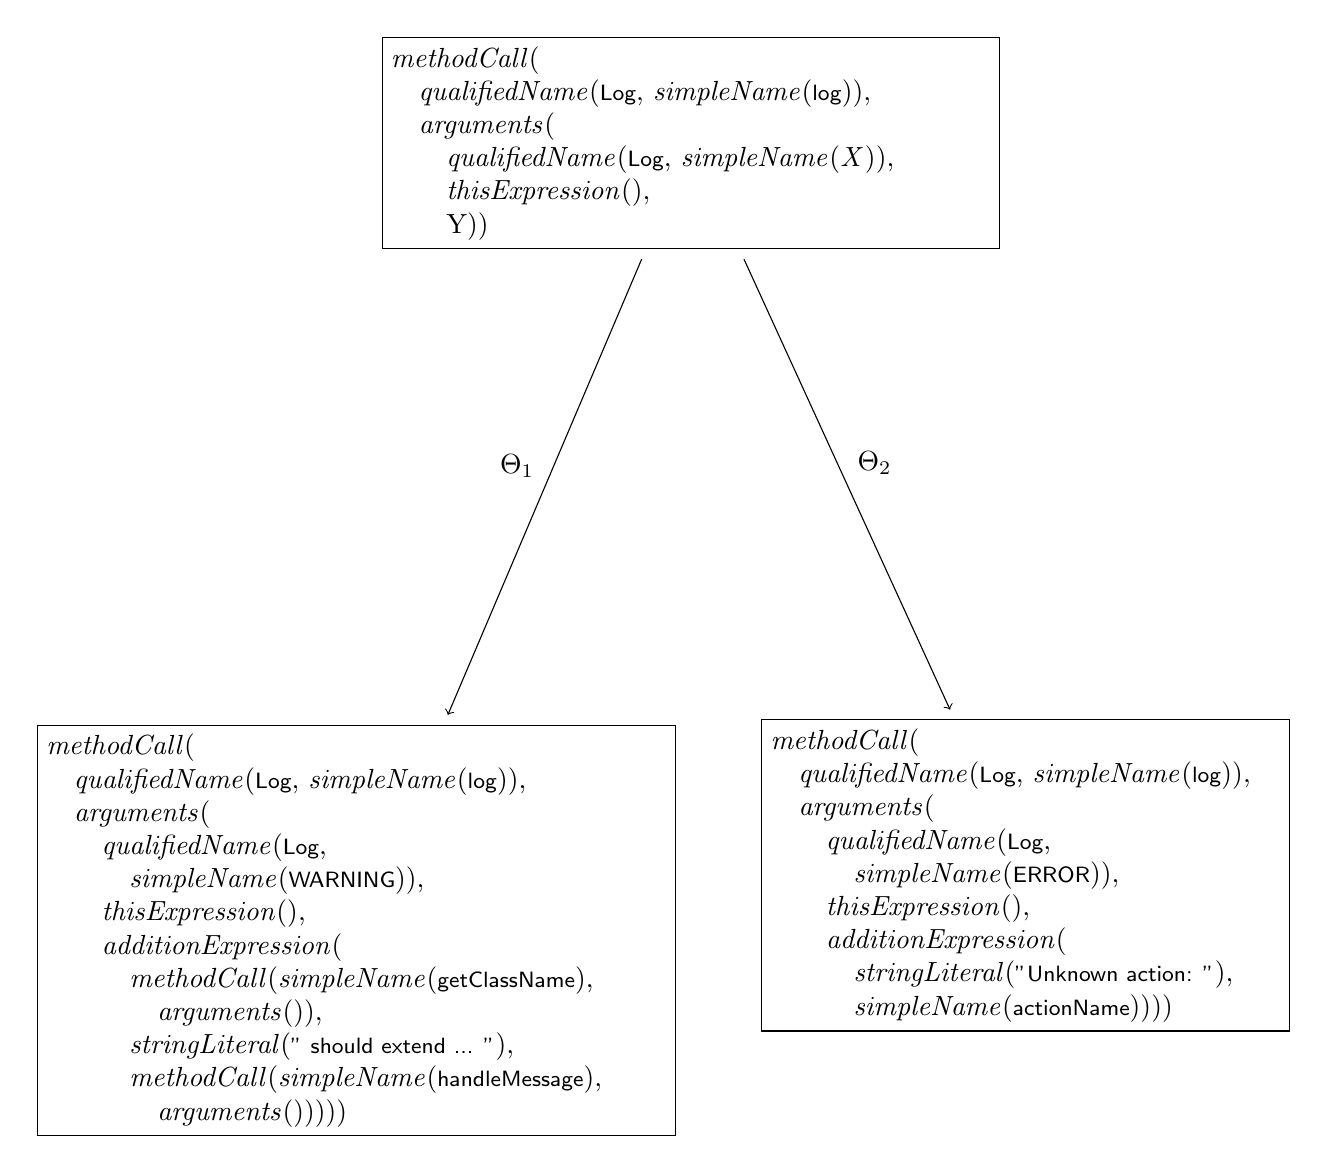
\begin{tikzpicture}
\node(a) at (4.25,10) {%
\fbox{\parbox[b][][b]{3in}{%
\text{\textit{methodCall}(}\\
\text{\hspace*{1em}\textit{qualifiedName}(\textsf{\footnotesize Log}, \textit{simpleName}(\textsf{\footnotesize log})),}\\
\text{\hspace*{1em}\textit{arguments}(}\\
\text{\hspace*{2em}\textit{qualifiedName}(\textsf{\footnotesize Log}, \textit{simpleName}(\textit{X})),}\\
\text{\hspace*{2em}\textit{thisExpression}(),}\\
\text{\hspace*{2em}Y))}}}%
};
\node(b) at (0,0) {%
\fbox{\parbox[t][][b]{3.1in}{%
\text{\textit{methodCall}(}\\
\text{\hspace*{1em}\textit{qualifiedName}(\textsf{\footnotesize Log}, \textit{simpleName}(\textsf{\footnotesize log})),}\\
\text{\hspace*{1em}\textit{arguments}(}\\
\text{\hspace*{2em}\textit{qualifiedName}(\textsf{\footnotesize Log},}\\ \text{\hspace*{3em}\mbox{\textit{simpleName}(\textsf{\footnotesize WARNING})}),}\\
\text{\hspace*{2em}\textit{thisExpression}(),}\\
\text{\hspace*{2em}\textit{additionExpression}(}\\
\text{\hspace*{3em}\textit{methodCall}(\textit{simpleName}(\textsf{\footnotesize getClassName}),}\\ \text{\hspace*{4em}\textit{arguments}()),}\\
\text{\hspace*{3em}\textit{stringLiteral}(\textsf{\footnotesize " should extend ... "}),}\\
\text{\hspace*{3em}\textit{methodCall}(\textit{simpleName}(\textsf{\footnotesize handleMessage}),}\\ \text{\hspace*{4em}\textit{arguments}()))))}}}%
};
\node(c) at (8.5,0.7) {%
\fbox{\parbox[t][][b]{2.55in}{%
\text{\textit{methodCall}(}\\
\text{\hspace*{1em}\textit{qualifiedName}(\textsf{\footnotesize Log}, \textit{simpleName}(\textsf{\footnotesize log})),}\\
\text{\hspace*{1em}\textit{arguments}(}\\
\text{\hspace*{2em}\textit{qualifiedName}(\textsf{\footnotesize Log},}\\ \text{\hspace*{3em}\mbox{\textit{simpleName}(\textsf{\footnotesize ERROR})}),}\\
\text{\hspace*{2em}\textit{thisExpression}(),}\\
\text{\hspace*{2em}\textit{additionExpression}(}\\
\text{\hspace*{3em}\textit{stringLiteral}(\textsf{\footnotesize "Unknown action: "}),}\\
\text{\hspace*{3em}\textit{simpleName}(\textsf{\footnotesize actionName}))))}}}%
};

\draw[->](a) -- (b) node[pos=0.5,above]{$\Theta_1\qquad$};
\draw[->](a) -- (c) node[pos=0.5,above]{$\qquad\Theta_2$};
\end{tikzpicture}
\end{small}
\caption{Anti-unification of the AUASTs of the logging calls in Examples 1 and 2.\label{fig:logging-anti}}
\end{figure}







%\section{Evaluation}\label{jigsaw-assessment}
\section{An Assessment of the Jigsaw framework}\label{jigsaw-assessment}
%\section{The Correspondence tool} \label{correspondenceTool}
%
%\RW{Describe here the procedure you used to select the examples, etc., how you tested Jigsaw, and what your findings were. At some point, you complained that Cottrell had not done something right ... do you have any evidence to demonstrate it?  How does this affect your work?  Such points can go in a discussion section towards the end of this chapter if they don't fit otherwise.  Full details of examples can go in an appendix; here, just describe enough so people can get the point.}
%
%\NZ{I think this experiment is not much about evaluating Jigsaw (The evaluation was conducted by Cottrell), but it is more about understanding what Jigsaw does and how to use it for my application . What I have mentioned was about detecting relevance links which is not related to my work. During my development, I added some statements to Jigsaw for the cases that was not covered in his work completely (e.g, Jigsaw did not detect the correspondence between inner type declarations of two nested type declarations when comparing the two upper type declarations }
%
%

%\name{Jigsaw} is a proof-of-concept implementation of the proposed approach to determining potential structural correspondences, which takes two AST nodes is an Eclipse plug-in that inputs a \name{Java} program, extracts ASTs of logged methods in it using the Eclipse JDT framework, applies a part of the implementation of Jigsaw to identify structural correspondences between ASTs in a pairwise manner and reuses the Jigsaw similarity function to measure the similarity between nodes involved in each correspondence connection.


To validate the effectiveness of the proposed approach by \citet{2008:fse:cottrell}, I applied the Jigsaw framework to compare the ASTs of a sample set of logged methods selected from a real-world software system in a pairwise manner and construct the CASTs of each pair.
%Jigsaw or correspondence???


%chapter{Experimental Studies}  \label{studies}
%To evaluate our approach, we have implemented a tool, and conducted three empirical studies on a set of LMs extracted from a real-world software system. In this section, we describe our experimental setup, present our studies, and discuss the results.



%the correspondence tool as
%\subsubsection{Experimental Setup}  \label{study1_setup}
\subsection{Setup}  \label{study1_setup}
%Our tool is a plug-in to the Eclipse integrated development environment (IDE) that implements our algorithm. The tool consists of three main components: a correspondence tool, an antiunifier-building tool, and a clustering tool. The correspondence tool inputs a pair of LMs, uses the Jigsaw framework to determine potential correspondences between their AST nodes, and outputs the generated CASTs and the Jigsaw similarity between them. The antiunifier-building tool inputs a pair of LMs, applies our anti-unification algorithm to construct an anti-unifier with a special attention to logging calls, and outputs the detailed view of anti-unifier and similarity measure (as described in Section~\ref{meth-antiUnifier}). The clustering tool inputs a set of LMs, applies a hierarchical clustering algorithm to classify them based on the similarity measurement, and outputs the detailed view of the generated anti-unifier for each cluster (as described in Section~\ref{meth-clustering}).
% figure of architecture?

As a subject for my study, I used \name{jEdit}, a programmer's text editor tool written in \name{Java} programming language. I chose this subject because it is a real program that has been used constantly by many developers, and it employs real usage of logging calls. My tool extracts all LMs within the source code of this program using the Eclipse JDT framework. However, a subset of them was selected containing 9 LMs that showed varying levels of similarity on manual examination, and it has been used as a test suite throughout this study (see Table~\ref{table:ljms}). The \code{EditBus.send(..)} method contains two logging calls. To handle this case we split it into two cases: case 3 contained the first logging call while the second one was removed; case 4 contained only the second logging call. We will describe our approach for LMs containing multiple logging calls in details in Section~\ref{meth-multipleLogs}. The last three LMs were manually modified by adding some statements for the sake of dealing with important cases that we otherwise would have missed testing. Case 8 simulates the addition of an \code{if}-statement that formed a nested \code{if}-statement enclosing a logging call. Cases 9 and 10 simulate the addition of statements to improve the test coverage.


\begin{figure} [H]
  \centering
  \begin{tabular}{clc}
    \toprule
    Case & Logged methods & Size (LOC)\\
    \midrule
    1& {PluginJAR.generateCache()} &104\\
    2& {MiscUtilities.isSupportedEncoding(..)} &9\\
    3& {EditBus.send(..)} &14\\
    4& {EditBus.send(..)}* &14\\
    5& {EditAction.Wrapper.actionPerformed(..)} &5\\
    6& {EBPlugin.handleMessage(..)} &6\\
    7& {BufferHistory.RecentHandler.doctypeDecl(..)} &3\\
    8& {JARClassLoader.loadClass(..)} &32\\
    9& {VFS.DirectoryEntry.RootsEntry.rootEntry(..)} &36\\
    10& {ServiceManager.loadServices(..)} &20\\
    \bottomrule
  \end{tabular}
  \caption[Logged methods used as our test suite.]{Logged methods used as our test suite; all are contained in the \protect\name{org.gjt.sp.jedit} package with the exception of case 9 that is in the \protect\name{org.gjt.sp.jedit.io} package.}
  \label{table:ljms}
\end{figure}



%\subsubsection{Setup}  \label{study1-setup}
The jigsaw framework was used to compare LMs of the test suite in a pairwise manner (55 test cases in total, including self-comparisons) and to produce the CASTs of each pair. The Jigsaw similarity was also measured for each of these test cases.
I examined the generated CASTs of these test cases and selected a subset of 4 cases with various levels of correspondences as depicted in the Table~\ref{jigsaw_4_test_cases}. Case 1 contains the comparison of a \name{Java} element with itself. Case 2 contains the comparison of two \name{Java} elements that are both syntactically and semantically dissimilar.  Case 3 contains the correspondence between two \name{Java} elements that are syntactically dissimilar but are semantically relevant. Case 4 contains the comparison of a logging call with another \name{Java} element that is not logging call but is syntactically relevant.




\begin{figure}
  \centering
  \begin{tabular}{clc}
    \toprule
    \shortstack{Test\\case} & \name{Java} source code fragment & \shortstack{Jigsaw\\similarity}\\
    \midrule

    \multirow{2}{*}{{1}}&{Log.log(Log.WARNING,this,"Unknown action: " + actionName);}& \multirow{2}{*}{1}\\

                         &{Log.log(Log.WARNING,this,"Unknown action: " + actionName);}\\
    \midrule

       \multirow{2}{*}{2}&{return entry;}& \multirow{2}{*}{0}\\
       &{int i=0;}\\
    \midrule


 \multirow{2}{*}{3}&
 /for (int i=0; i < comps.length; i++) {...}/&\multirow{2}{*}{\RW{???}}\\


      &
/while (entries.hasMoreElements())  { ...}/
      \\
    \midrule

    \multirow{2}{*}{4}&{Log.log(Log.WARNING,this,"Unknown action: " + actionName);}& \multirow{2}{*}{0.33}\\
      &{EditBus.removeFromBus(this);}\\
    \bottomrule

  \end{tabular}
  \caption{Results from examining the Jigsaw similarity for 4 sample \name{Java} source code fragment pairs.}
  \label{jigsaw_4_test_cases}
\end{figure}




\subsection{Results}  \label{study1-results}
The results of the pairwise comparison between LMs of the test suite is visualized in Figure~\ref{fig:jigsaw_graph}. As it is shown, the Jigsaw similarity for all self-comparisons is 1, while the level of Jigsaw similarity is different for pairs containing distinct LMs as our manual examination.

\begin{figure} [H]
  \centering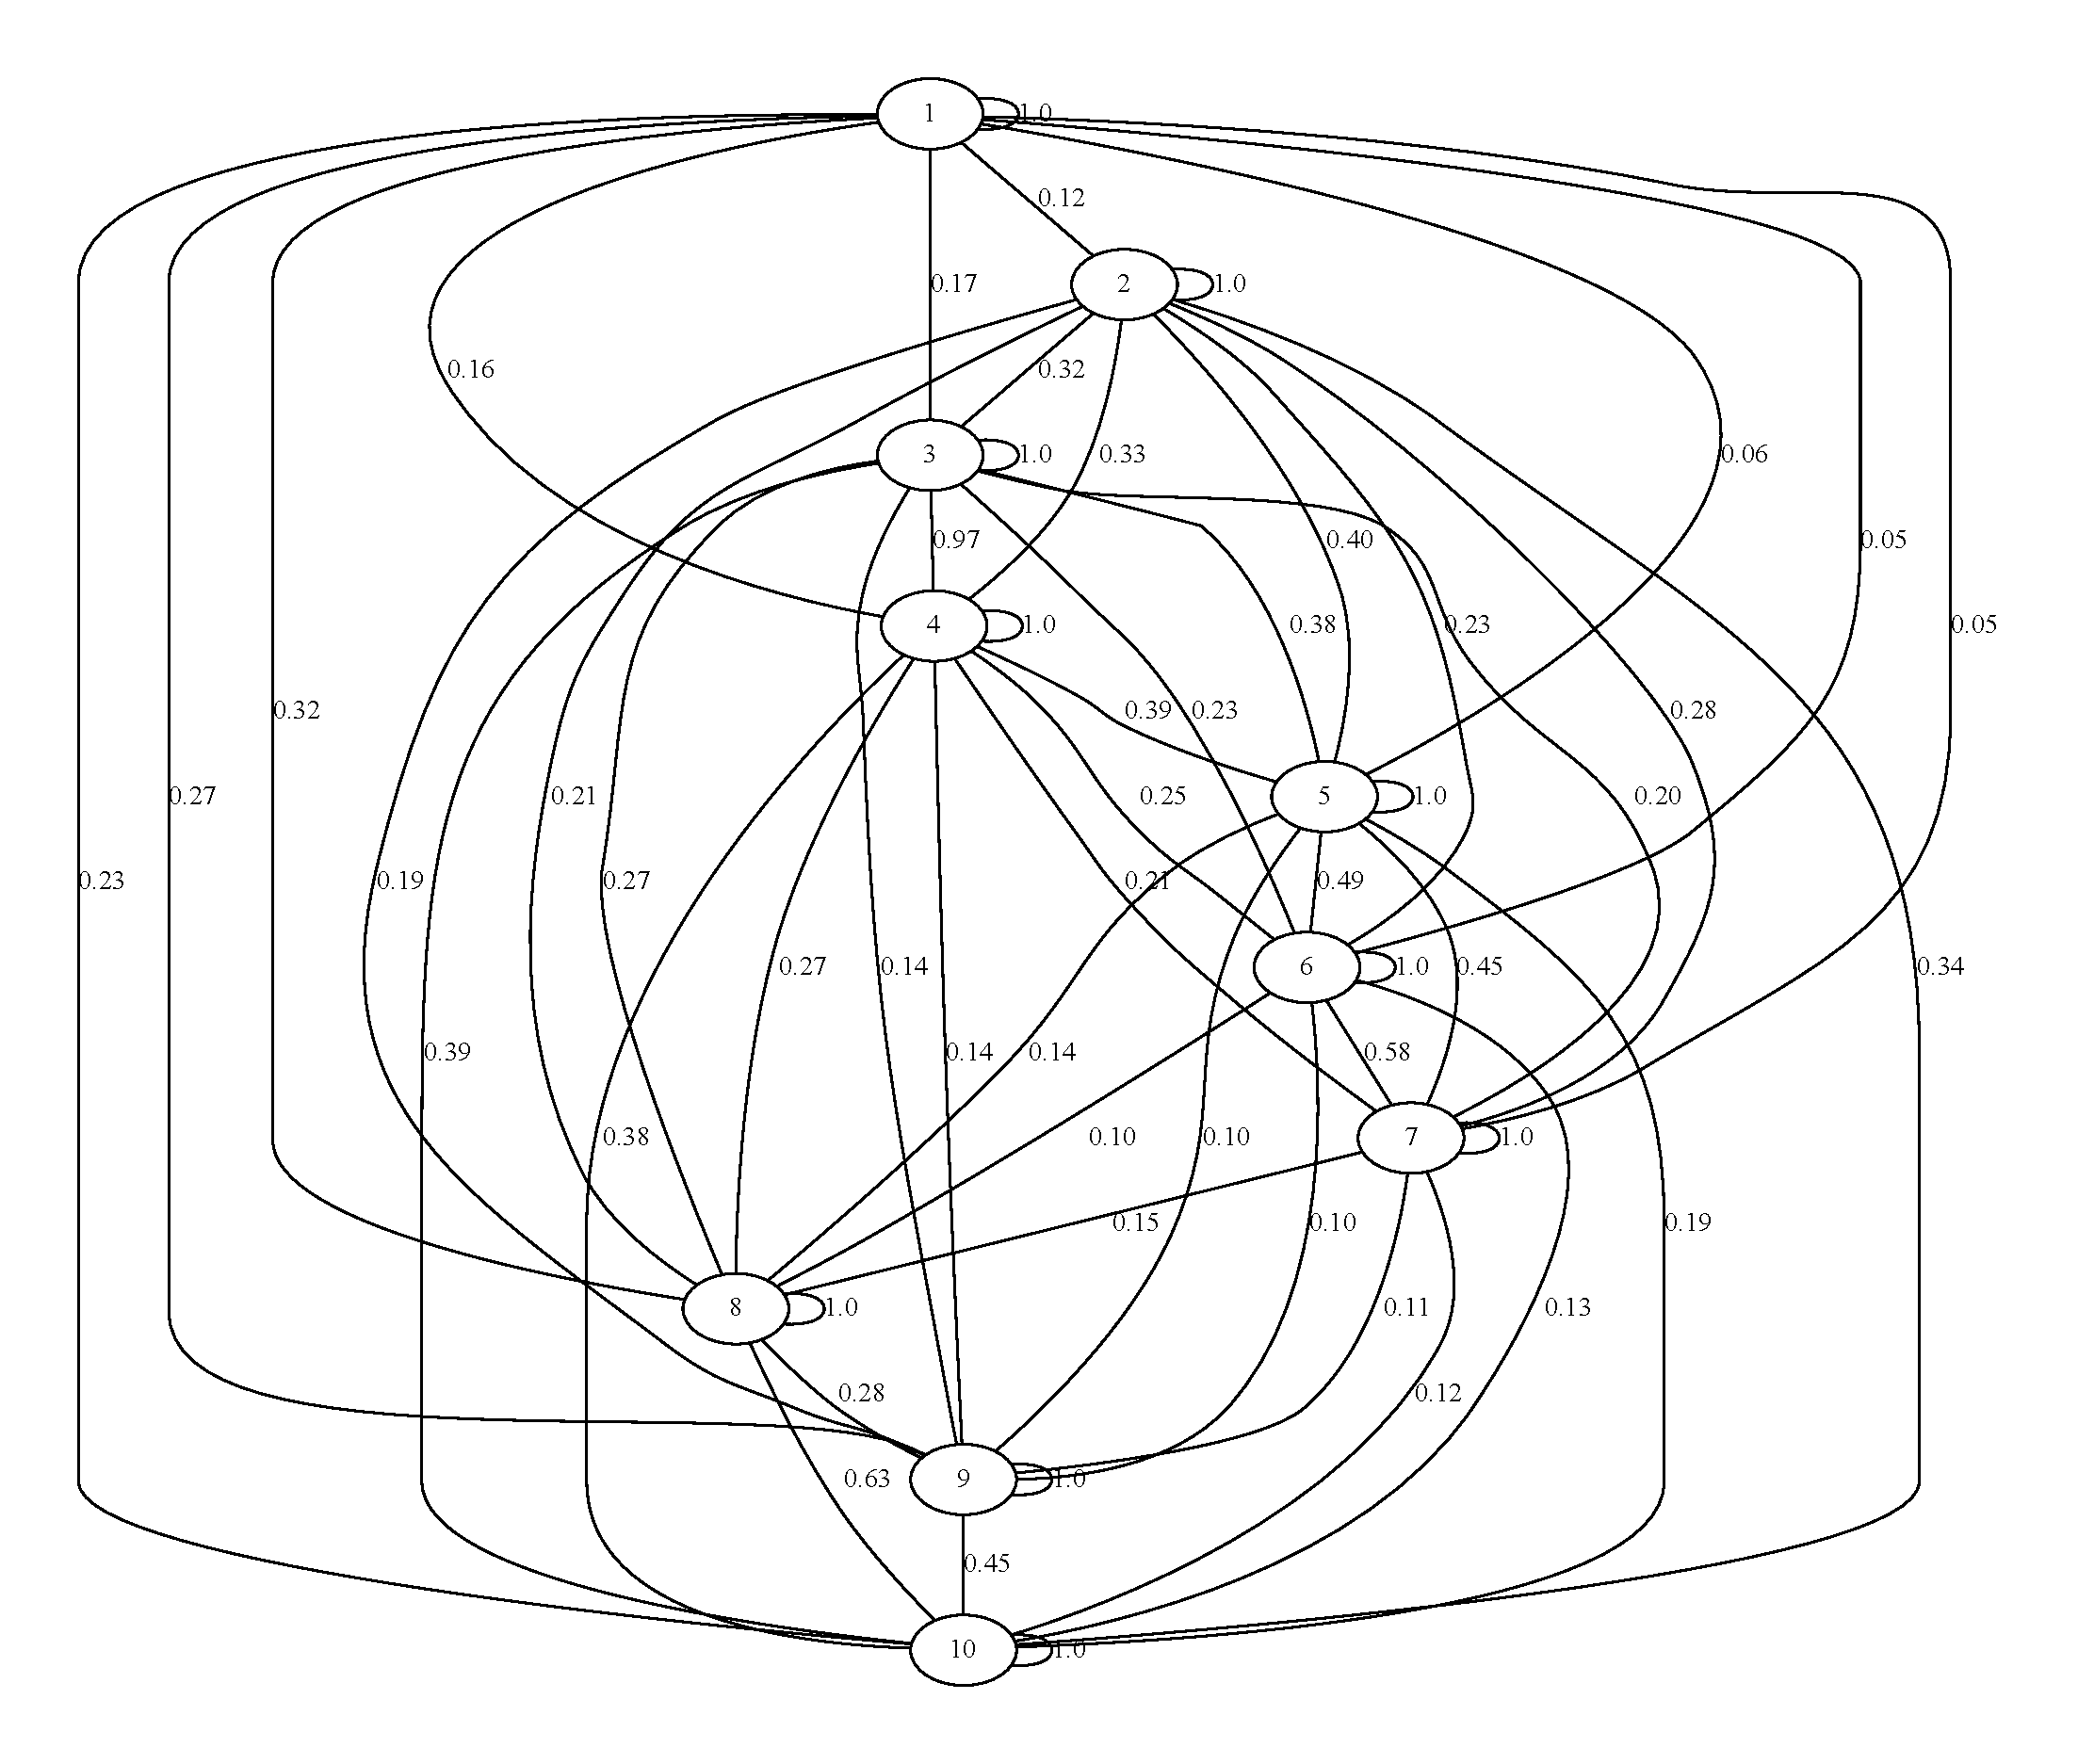
\includegraphics [width = \textwidth]{graphviz/jigsaw.pdf}
  \caption{A similarity graph representing pairwise Jigsaw similarities between LMs shown in Table~\ref{table:ljms}.}
  \label{fig:jigsaw_graph}
\end{figure}


The analysis of the 4 cases is shown in Table~\ref{jigsaw_4_test_cases}. Case 1 shows that a \name{Java} element that is compared with itself has a Jigsaw similarity of 1. Case 2 indicates that no correspondence connection is created when a \name{Java} element is compared with another \name{Java} element that is utterly dissimilar. Case 3 indicates that the similarity between a \code{for}-statement and a \code{while}-statement is non-zero, and that Jigsaw is able to detect semantic correspondences between \name{Java} elements. Case 4 shows that a logging call has non-zero similarity with another \name{Java} element that is not a logging call but is syntactically relevant. This case will be handled via the removal of this kind of correspondence connection, as will be described in Section~\ref{best-corr}. %\RW{Section???}


%\section{Comparison with the Jigsaw tool}  \label{comparison-Jigsaw}


\section{Summary}  \label{summary}
I described the approach proposed by \citet{2008:fse:cottrell} to determining structural correspondences between AST nodes using a similarity measure. I assess the functionality of their approach to address the problem through an empirical study that uses the Eclipse JDT framework for extracting the ASTs of a sample set of LMs selected from a real-world software system, and applies the Jigsaw framework for constructing the correspondence structures.




%Eclipse JDT as a concrete framework that can be used to manipulate ASTs of a source code written in the \name{Java} programming language. I also introduced Jigsaw, an existing framework for determining structural correspondences between AST nodes and measuring similarity between them.

%In this chapter, we described anti-unification as a technique to construct a common generalization of two given terms. We have also introduced an extended form of anti-unification, which is called higher-order anti-unification modulo theories, where a set of equivalence equations can be applied on higher-order extended structures to incorporate background knowledge. In addition, we provided a brief description of AST that maps \name{Java} source code in a tree structure form, and why an extended form of it, named AUAST, is required to create higher-order structures specific to our problem context. Finally, we discuss the Jigsaw framework and how it could assist us in determining the potential structural correspondences. 